\chapter{显微图像处理平台系统设计}
%
%本设计中采用了树莓派板 ARM 处理器,运用板中的 CSI-2 串行接口,将 IMX135 相机采集的显微图像传输至 BCM2836 处理器,在图像处理器 GPU 中进行数据的编 解码,对图像进行降噪、图像增强等处理,并以 H.264 格式的视频格式存储在 SD 卡 上,并通过 HDMI 接口在显示器上播放显示,采用基于误差修正的算法对图像进行 缺损检测。树莓派板的硬件框图系统如图\ref{fig:rasp_1} 所示。
这一图像处理平台使用了基于 RESTful 架构的开放 API 体系,通过统一的 Web 服务展现给用户,借用PaaS平台完成部分存储和归档功能。借助浏览器获取相关的信息。借助树莓派较多的硬件接口,充分调用相关功能\cite{restful}。

\begin{figure}[h]
\centering
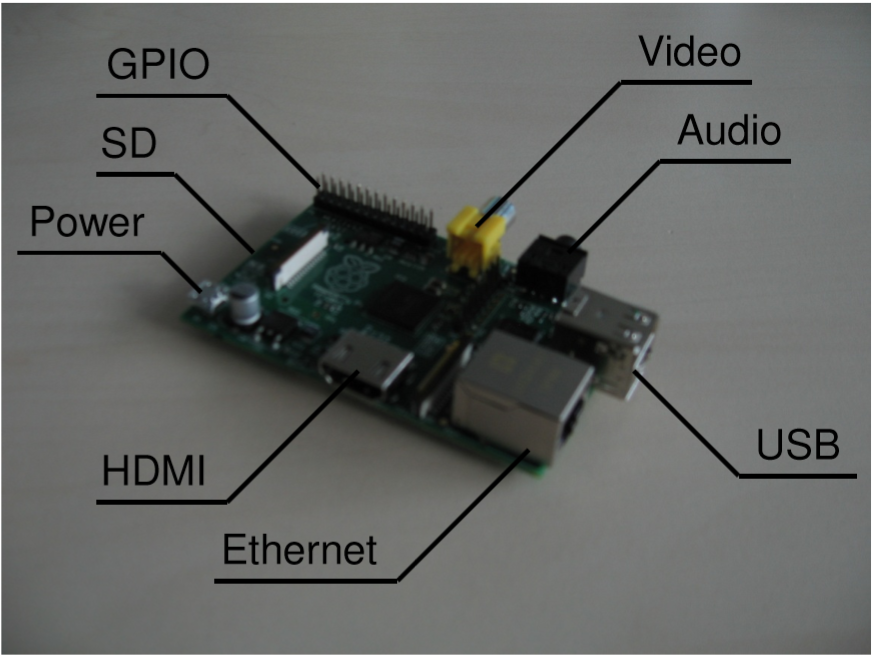
\includegraphics[width=0.7\linewidth]{Figure/rasp_1}
\caption{树莓派实物和接口}
\label{fig:rasp_3}
\end{figure}


\section{树莓派平台简介}
Raspberry Pi(中文名为“树莓派”,简写为 RPi,或者 RasPi/RPi)是为学生计算机编程教育而设计,只有信用卡大小的卡片式电脑,其系统基于 Linux。
树莓派由注册于英国的慈善组织“Raspberry Pi 基金会”开发,Eben Upton 埃·厄普顿为项目带头人。2012 年 3 月,英国剑桥大学埃本·阿普顿(Eben Epton)正式发售世界上最小的台式机,又称卡片式电脑,外形只有信用卡大小,却具有电脑的所有基本功能,称为Raspberry Pi 电脑板,中文译名"树莓派"。这一基金会以提升学校计算机科学及相关学科的教育,让计算机变得有趣为宗旨。基金会期望这 一款电脑无论是在发展中国家还是在发达国家,会有更多的其它应用不断被开发出来,并应用到更多领域\cite{raspHDMI}\cite{rasphome}。

通过装载相应的 Linux 系统和相应的应用程序,RaspberryPI可以实现强大的通用能力,还具有廉价、体积小等优点. 以硬件开源的嵌入式系统树莓派作为应用开发平台,通过TCP /IP 协议实现了数据查看的便捷化; 便于联网的浏览器可以随时监看图片。

\begin{figure}[h]
\centering
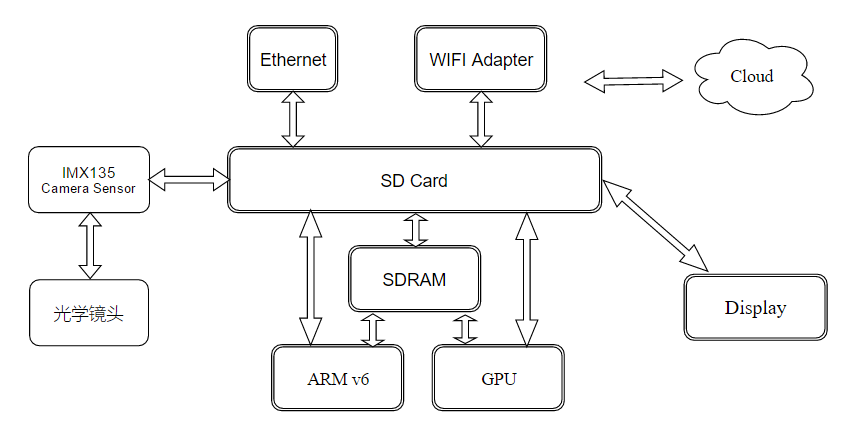
\includegraphics[width=0.7\linewidth]{Figure/rasp_arch_1}
\caption{显微平台数据流向}
\label{fig:rasp_arch_1}
\end{figure}


整体的数据流图如图\ref{fig:rasp_arch_1}所示,拍摄物体经过光学镜头聚焦成像处理后,相应成像信息反映到IMX135的CMOS传感器中,经过CPU和GPU的处理后,存储在SD卡中,后联网存储备份归档在云中,同时还输出桌面显示,通过浏览器的方式完成图像的浏览和输出。


\section{图像传感器接口驱动程序}
\subsection{接口驱动简介}
V4L(Video4Linux)是为市场现在常见的电视捕获卡和并口及USB口的摄像头提供统一的编程接口。同时也提供无线电通信和文字电视广播解码和垂直消隐的数据接口。V4L2是V4L的改进版。从编程的角度来看V4L2,作为Linux内核中关于视频设备的框架子系统,对于上层应用提供了一套统一的接口来访问底层的视频设备,起到抽象底层硬件的差异的作用。向下面向视频采集设备的驱动开发定义了一套开发规范,同时提取出公共代码避免代码冗余,将所有的视频采集设备的驱动程序都纳入其的管理之中。V4L2不仅给驱动程序编写者带来极大的方便,同时也方便了应用程序的编写和移植,在远程会议、可视电话、视频监控系统和嵌入式多媒体终端中都有广泛的应用\cite{v4l2embedded}。
Linux系统V4L2的能力可在Linux内核编译阶段配置,默认情况下都有此开发接口。V4L2从Linux 2.5.x版本的内核中开始出现。

应用程序通过V4L2接口采集视频数据分为五个步骤:

首先,打开视频设备文件。

其次,进行视频采集的参数初始化,通过V4L2接口设置视频图像的采集窗口、采集的点阵大小和格式;

第三,申请若干视频采集的帧缓冲区,并将这些帧缓冲区从内核空间映射到用户空间,便于应用程序读取/处理视频数据;

第四,将申请到的帧缓冲区在视频采集输入队列排队,并启动视频采集;

第五,驱动开始视频数据的采集,应用程序从视频采集输出队列取出帧缓冲区,处理完后,将帧缓冲区重新放入视频采集输入队列,循环往复采集连续的视频数据;

第六,停止视频采集。

第七,关闭视频设备文件。

简要查看下对结构体$v4l2_format$的情况,其由type和联合体fmt构成,来描述视频设备当前行为和数据的格式。
v4l2的struct展示在附录中:

%\lstinputlisting[language=C,caption={V4L2 struct format Code},label=c]{./Code/v4l2.h}



\section{显微图像预处理}
\subsection{预处理图像算法研究分析}
预处理的目的是为了消除过度曝光、不合理的对比度、图像扭曲以及噪音等因素。在图像输出的部分,由于之前所说的因素,图像最终往往难以清晰。为了弥补,保证处理算法对指纹图像具有足够的鲁棒性,图像增强是是其中需要的一点。图像增强是对图像采用一定的算法进行处理,使其缺陷的结构清晰,进而突出和保留固有的缺陷图像而避免与噪声混淆\cite{imageprocessing}。
\subsubsection{线性插值}
线性内插值算法描述如下:
对于一个目的像素,设置坐标通过反向变换得到的浮点坐标为(i+u,j+v) (其中i、j均为浮点坐标的整数部分,u、v为浮点坐标的小数部分,是取值[0,1)区间的浮点数),则这个像素得值 f(i+u,j+v) 可由原图像中坐标为 (i,j)、(i+1,j)、(i,j+1)、(i+1,j+1)所对应的周围四个像素的值决定,即:
\begin{equation}
\label{chazhi}
f(i+u,j+v) = (1-u)(1-v)f(i,j) + (1-u)vf(i,j+1) + u(1-v)f(i+1,j) + uvf(i+1,j+1)  
\end{equation}


其中式\ref{chazhi}中$f(i,j)$表示源图像$(i,j)$处的的像素值,以此类推。
如下面公式所示。


\begin{center}
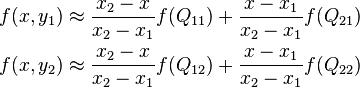
\includegraphics[width=0.7\linewidth]{Figure/figureline_1}
\end{center}


\subsubsection{中值滤波法}
中值滤波法是一种非线性平滑技术,它将每一像素点的灰度值设置为该点某邻域窗口内的所有像素点灰度值的中值.中值滤波是基于排序统计理论的一种能有效抑制噪声的非线性信号处理技术,中值滤波的基本原理是把数字图像或数字序列中一点的值用该点的一个邻域中各点值的中值代替,让周围的像素值接近的真实值,从而消除孤立的噪声点。方法是用某种结构的二维滑动模板,将板内像素按照像素值的大小进行排序,生成单调上升(或下降)的为二维数据序列。由此二维中值滤波输出为g(x,y) =med{f(x-k,y-l),(k,l∈W)} ,其中,f(x,y),g(x,y)分别为原始图像和处理后图像。W为二维模板,通常为33,55区域,也可以是不同的的形状,如线状,圆形,十字形,圆环形等。
\begin{figure}[h]
\centering
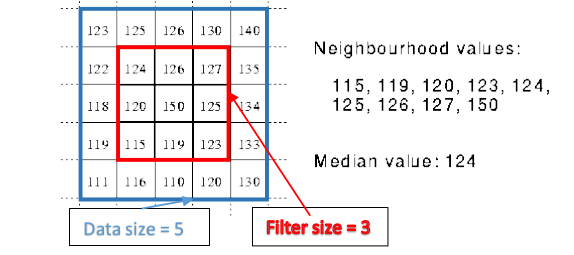
\includegraphics[width=0.7\linewidth]{Figure/median_2}
\caption{中值滤波三三法}
\label{fig:median_1}
\end{figure}

通过上面的介绍,我们简单的了解了图像预处理中的滤波算法。通过比较两种滤波算法,在 ARM 中进行图像预处理时,可以看出,虽然中值滤波算法复杂度更大, 但其滤波的效果更佳,同时树莓派中的 GPU 运算速度又很高,因此采用中值滤波进 行图像预处理,可以在 GPU 内部进行数学运算,这对于提高图像处理能力提供了巨 大帮助,因此在本项目中,由于均值滤波会使图像的边缘信息丢失,不利于显微系统 精度检测的提高,因此采用了中值滤波算法对该系统的图像做了预处理。

\section{实时图像处理算法分析}
由于本系统是靠显微镜来保证对准精度,进而提高测量精度的,因此,受显
微镜观测视场的限制,无法直接观察大尺寸范围的物体。为了实现大尺寸
样品的观测,就需要采用图像拼接技术,将采集到的多幅图像进行拼接,
在进行图像融合时,设定一个图像局部清晰度的判定标准,本文中采用 图像灰度均匀值作为标准,选择采集的比较高清晰的显微图像,尽量减少原图质量对 融合效果的影响,再对显微图像进行区域分块,尽量将图像清晰和模糊的区域分割开 来。将观测视场临近的两幅图像分割出来的清晰区域块进行带权值的像素融合,以此类推,扩展到将所有的视场相邻的显微图进行融合,从而得到一个较大视场内的显微图像\cite{fastprocessing}。 

图像分割在对象定位、对象识别、视觉跟踪、图像检索和
图像理解等各种应用中属于至关重要的步骤,其
准确率和执行效率直接影响到后续步骤中目标特征提取和识别任务的效果。根据实现策略不
同,图 像 分 割 算 法 主 要 有 阈 值 法、模板匹配、聚类
、活动边缘模型、图切割模型和区域
增长等几种。这几种算法
这几种算法在特定的应用领域都有各自的优势特点,但均很
难在分割正确率和执行效率两个衡量图像分割方
法优劣的核心指标上同时都取得最佳性能,往往
只能侧重其中之一,通常都是在两者之间寻找某
种折衷。这里选用阈值分割来衡量匹配的阈值节点\cite{fenge}。


在对光学薄膜表面缺陷检测时,把图像中的缺陷进行阈值分割十分必要,一幅图像通常由前景区域和背景区域组成。图像分割的目的是将背景区域和前景区域分开,提高特征提取的准确性,同时节省处理时间,从而提高整个系统的性能。若选取
的分割阈值过高的话,图像缺陷会被掩盖在背景中,会导致图像表面缺陷的漏检;相 反,若阈值选取太低的话,一部分背景就会被误判为图像存在的缺陷。图像的阈值分割利用了图像中要提取的目标物与其背景在灰度特性上的差
异,把图像视为具有不同灰度级的两类区域(目标和背景)的组合,选取一个合
适的阈值,以确定图像中每一个像素点应该属于目标还是背景区域,从而产生相应的二值图像\cite{guleialgo}。



\section{上位机图像显示处理}
树莓派预搭载的编程开发环境是 Python 语言。 Python 是一种面向对象、直译式计算机编程
语言,已有近20 年的发展历史,包含了一组完善而且容易理解的标准库,能够轻松完成很多常见
的任务,语法简捷、清晰,且具有垃圾回收功能,能够实现内存的自动管理,常用于处理系统管理
任务和网络程序编写,也适合完成各种高级任务。Python经常被用于Web开发,Python对于各种网路协定的支援很完善,因此经常被用于编写服务器软件、网路蠕虫。第三方函式库Twisted支援非同步线上编写程式和多数标准的网路协定(包含客户端和服务器),并且提供了多种工具,被广泛用于编写高性能的服务器软件。另有gevent这个流行的第三方库,同样能够支持高性能高并发的网络开发\cite{raspnet}。
在显示上主要考虑下面的几种框架或库\cite{rasgpio}。

\subparagraph{Django}
Django是一个开放原始码的Web应用框架,由Python写成。採用了MVC的软体设计模式,即模型M,视图V和控制器C。
使用 Django 最大的好处就是包括资料库的连接、 表单、登入系统、管理界面等等建构网站应该要有的元件都是 Django 本身的一部份,虽然乍看之下失去了一些弹性,但是却可以加快开发效率,简化组件复用工作量。

\subparagraph{Qt}
Qt是一个跨平台的C++应用程序开发框架。广泛用于开发GUI程序,这种情况下又被称为部件工具箱。也可用于开发非GUI程序,比如控制台工具和服务器。Qt使用标准的C++和特殊的代码MOC生成扩展以及一些宏。
\subparagraph{GTK+}
GTK+ 最初是 GIMP 的专用开发库 (GIMP Toolkit),后来发展为Unix-like系统下开发图形界面的应用程序的主流开发工具之一。GTK+是自由软件,并且是GNU计划的一部分。GTK+的许可协议是LGPL。GTK+使用C语言开发,但是其设计者使用面向对象技术。也提供了C++(gtkmm)、Perl、Ruby、Java 和 Python ( PyGTK ) 绑定,其他的绑定有Ada、D、Haskell、PHP和所有的.NET编程语言。


考虑到目前多类型的跨客户端的平台化趋势,注重系统的可迁移,决定在B/S架构的基础上使用默认的编程开发环境Python,并使用Django框架降低开发难度,不考虑CGI的从头书写,和本地的系统C/S平台,如需要直接在系统平台内操作系统上的文件管理查看即可\cite{rasptcpip}。

\section{本章小节}
本章主要简单介绍了树莓派平台的基本结构,常见应用。分析了驱动程序V4L2的特性和使用,了解图像预处理的方式,包括线性插值、中值滤波和高斯滤波等。了解了图像处理中的聚类和分割。最后对图像显示的几种常见的方式做了介绍,最后选定使用Django的框架来进行快速的开发。